\section{System design}
I dette afsnit vil koncepterne bag mange af de teknologier, der gør systemet muligt, blive belyst, men der vil også blive analyseret og diskuteret, hvordan systemet skal designes. Dette vil blive gjort ud fra hvordan kravspecifikationen bedst muligt vil blive opfyldt.
Systemet er for eksempel gennem kravspecifikationen pålagt både at være sikkert \ref{k:anonymt}, men samtidig også at skulle køre med en fornuftig indlæsnings tid \ref{k:load}. Disse krav modarbejder for det meste hinanden på flere forskellige måder, og er derfor relevante for forståelsen af processen, der leder op til det endelige system. Systemet er også beskrevet i det mere generelle indhold under afsnit \ref{produkt_beskrivelse}, og mere i dets fulde struktur senere under afsnit. \ref{Opsummering_Overvejelserne}

\subsection{Central eller decentral løsning}
\label{Central_De_loesning}
%Hvad er centraliceret system / decentraliceret
Løbende opdateringer, til et system for hemmelige beskeder over sociale medier, menes essentielle. F.eks. kunne de enkelte sociale medier til enhver tid nedlægge et sådan hemmeligt systems anvendte konti-bots, eller det enkelte sociale netværk kunne ændre deres generelle struktur, API eller ligende fra en dag til den næste.
% Centraliceret bot information
I dette system anvendes f.eks. flere dynamisk generede bots, til at sikre brugerens anonymitet, samt også til deres generelle kommunikation på platformen. Men grundet at de sociale medier generelt ikke ønsker systematisk genererede anonyme brugere på deres platform, og at disse bots desuden også kunne være associeret med en potentielt mistænkelig opførelse, vil en opdateret information om disse anvendte bots findes nødvendig.
% Opdaterings mulighed
Et centraliseret system åbner muligheden for dette, da et sådant system altid kan opdateres løbende, hvilket findes mere besværligt i et decentraliseret system. I et decentraliseret system kunne forskellige brugere, under et dynamisk udviklende miljø, nemlig ende med at være fastlåst med software, der potentielt er defekt, eller ville kræve at blive hentet på ny.
En sådan mulighed for løbende opdateringer, anses også mange gange for essentiel under en mulig skalering af systemer, blandt andet når systemets behov kræver større fundamentale re-designs, og er derfor ofte anvendt.
% Fokus på køretid
For dette projekts syn vil et større centraliseret system også anses for at være favorabelt, da dette potentielt vil øge hastighed ved brugerenes anvendelse. F.eks. kunne en centraliseret server indeholde en kortlægning af alle relevante opslag, og derved mindske de enkelte brugeres søgninger, eller mindske antallet af påkrævede anmodninger til de forskellige sociale medier. [Figur \ref{fig:CentralDatabaseList}]
% Fokus på sikkerhed 
Til gengæld, for samme i et decentraliseret system, kan en centrale server nemt spærres fra en tredjepart, og ville derfor være et vigtigt knudepunkt i systemet.

\begin{figure}[H]
    \begin{subfigure}{0.5\textwidth}
        \centering
        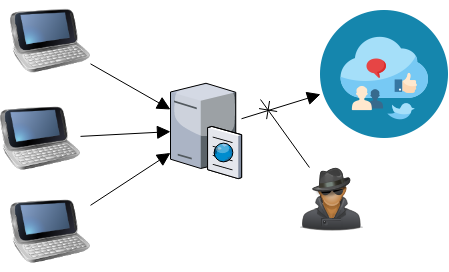
\includegraphics[width=1\linewidth, height=4cm]{Projectdoc/Assets/Illustrationer/Security_diagram_1.png} 
        \caption{Central server}
        \label{fig:central_server}
    \end{subfigure}
    \begin{subfigure}{0.5\textwidth}
        \centering
        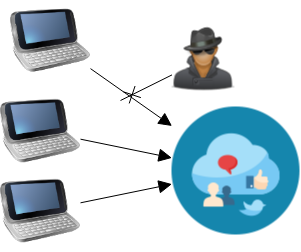
\includegraphics[width=0.7\linewidth, height=4cm]{Projectdoc/Assets/Illustrationer/Security_diagram_2.png}
        \caption{Klient-baseret system (decentral)}
        \label{fig:decentral_server}
    \end{subfigure}
    \caption{Forskellen på central og decentral server struktur}
    \label{fig:serverstruktur}
\end{figure}

Hvis projektet i stedet for hastighed skulle anse højere sikkerhed, ville et decentraliseret system, potentielt være at foretrække. 
Et decentraliseret system indeholder nemlig nødvendigvis ingen knudepunkter [Figur \ref{fig:central_server}], og et eventuelt system nedbrud eller informations lækage, ville derfor være mindsket, da der ikke findes et centralt brist.
Selvfølgelig ville enkelte del punkter, stadig have mulighed for at blive blokeret, men i sådanne tilfælde ville dette, kontra i et centraliseret system, ofte ikke blokere nogen større helhed [Figur \ref{fig:decentral_server}].

\begin{figure}[H]
    \begin{subfigure}{0.33\textwidth}
        \centering
        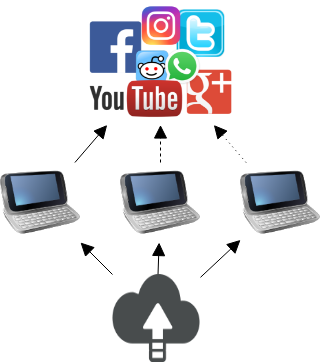
\includegraphics[width=0.7\linewidth, height=4cm]{Projectdoc/Assets/Illustrationer/Device_Opdate.png} 
        \caption{Lokale enheds kendte lister, opdateret via softwareopdateringer}
        \label{fig:DeviceOpdate}
    \end{subfigure}
    \begin{subfigure}{0.33\textwidth}
        \centering
        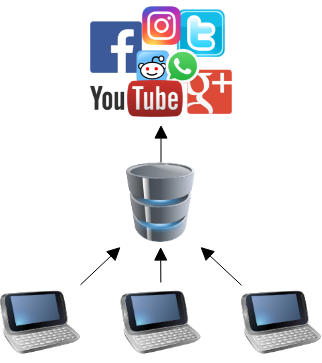
\includegraphics[width=0.7\linewidth, height=4cm]{Projectdoc/Assets/Illustrationer/CentralDatabase.png}
        \caption{Én central database}
        \label{fig:CentralDatabaseList}
    \end{subfigure}
    \begin{subfigure}{0.33\textwidth}
        \centering
        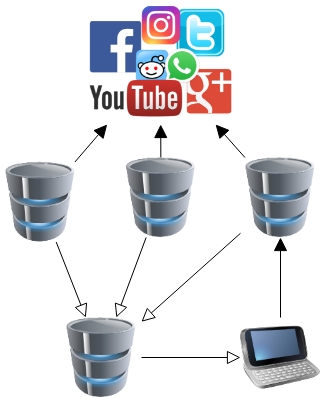
\includegraphics[width=0.7\linewidth, height=4cm]{Projectdoc/Assets/Illustrationer/MainDomainServer.png}
        \caption{Et netværk af databaser, kendt af enhederne, og opdateret fra en hoveddatabase}
        \label{fig:MainDomain}
    \end{subfigure}
    \caption{Forskellige medie kontakt former.}
    \label{fig:MedieContact}
\end{figure}

% Største centraliserings metode
Et centraliseret system kan dog stadig sikres yderligere. F.eks. kunne tilgangen fra de enkelte brugeres enheder mindskes, ved opsætning af en større database, dennes formålet udelukkende at indeholde information om mindre servere, der potentielt kunne indeholde mindre grupperinger, med informationen for de anvendte bots [Figur \ref{fig:MainDomain}]. Derved mindskes opmærksomheden på systemets centrale knudepunkt, da denne kun findes nødvendig at kontakte, hvis forbindelsen til de mindre ikke kan etableres, f.eks. ved en blokering. Denne struktur ville også mindske faren ved potentiel overvågning, da lækagen kun ville være gældende for de mindre partioner af systemet.
Samme funktionalitet kan selvfølgelig også opnås gennem et decentraliseret system, hvis man i stedet for at anvende en større server, opdaterede de enkelte klienter igennem system opdateringer [Figur \ref{fig:DeviceOpdate}]. Til gengæld vil dette øge de enkeltes mulighed for fejl, men man ville herved ikke kræve samme investering i hardware og vedligeholdelse deraf.

\subsection{Sammenkædning af beskederne}
Et større problem for anvendelses hastighed i projektets kommunikationsplatform, også omtalt i tidligere afsnit \ref{Central_De_loesning}, ses ved hentning af platformens forskellige sammenhængende beskeder, også kaldet tråde.\\
For at systemet, eller de enkelte brugere, skal kunne finde de beskeder tilhørende en sammenhæng, bliver et tiltænkt system for dette nødvendigt. Sådant et system må selvfølgelig ikke foregå på åbenlys vis, da dette ville kunne skabe en større kompromittering af systemet, og øger derfor vigtigheden af placeringen for disse informationer. Placering af denne information på eventuelt en hovedserver, ville også øge data trafikken mod disse servere, og derved højne deres synlighed. En løsning findes dog endeligt ved udnyttelse af metadata. F.eks. kunne en sammenhæng blive genereret ud fra en prædefineret algoritme, så som GPS-lokation, og derved give den sikrede kommunikationsplatform noget specifikt at søge efter under hentning, uden at vække større mistænkeligehed. 

%På projektets sikrede kommunikationsplatform vil det være nødvendigt at kunne finde sammenhængende beskeder, samtidig med at denne sammenkædning vil ikke kunne foregå på åbenlys vis på et socialt medie. I stedet kunne én mulighed være, at gemme sammenhængen i noget tilsyneladende uskyldig metadata, men at denne data er genereret ud fra en prædefineret algoritme. Dette vil give den sikrede kommunikationsplatform noget specifikt at søge efter, uden at det vil være et let læseligt flag. Men hvad er metadata?

\subsubsection{Metadata}
Metadata kan grundlæggende defineres som data om data. Dermed kan det anvendes i mange sammenhænge. Et eksempel kunne være et billede. Dataen i et billede er i simpleste forstand lysintensiteter, i sort/hvid billeder, eller farver. Men udover denne data, kunne man også gemme ting som dato, klokkeslet, GPS koordinater, navnet på ophavsmanden osv. Alt dette er eksempler på metadata, som ikke påvirker indholdet, men som gør indholdet mere brugbart i mange forskellige sammenhænge. For eksempel vil vedhæftede søgeord gøre et billede galleri meget mere effektivt i at præsentere det ønskede materiale. Metadata kan både genereres automatisk af hardware/software systemer, men en bruger kunne også tilføre metadata manuelt.

\begin{table}[H]
    \begin{minipage}{.65\textwidth}
        \begin{figure}[H]
            \centering
            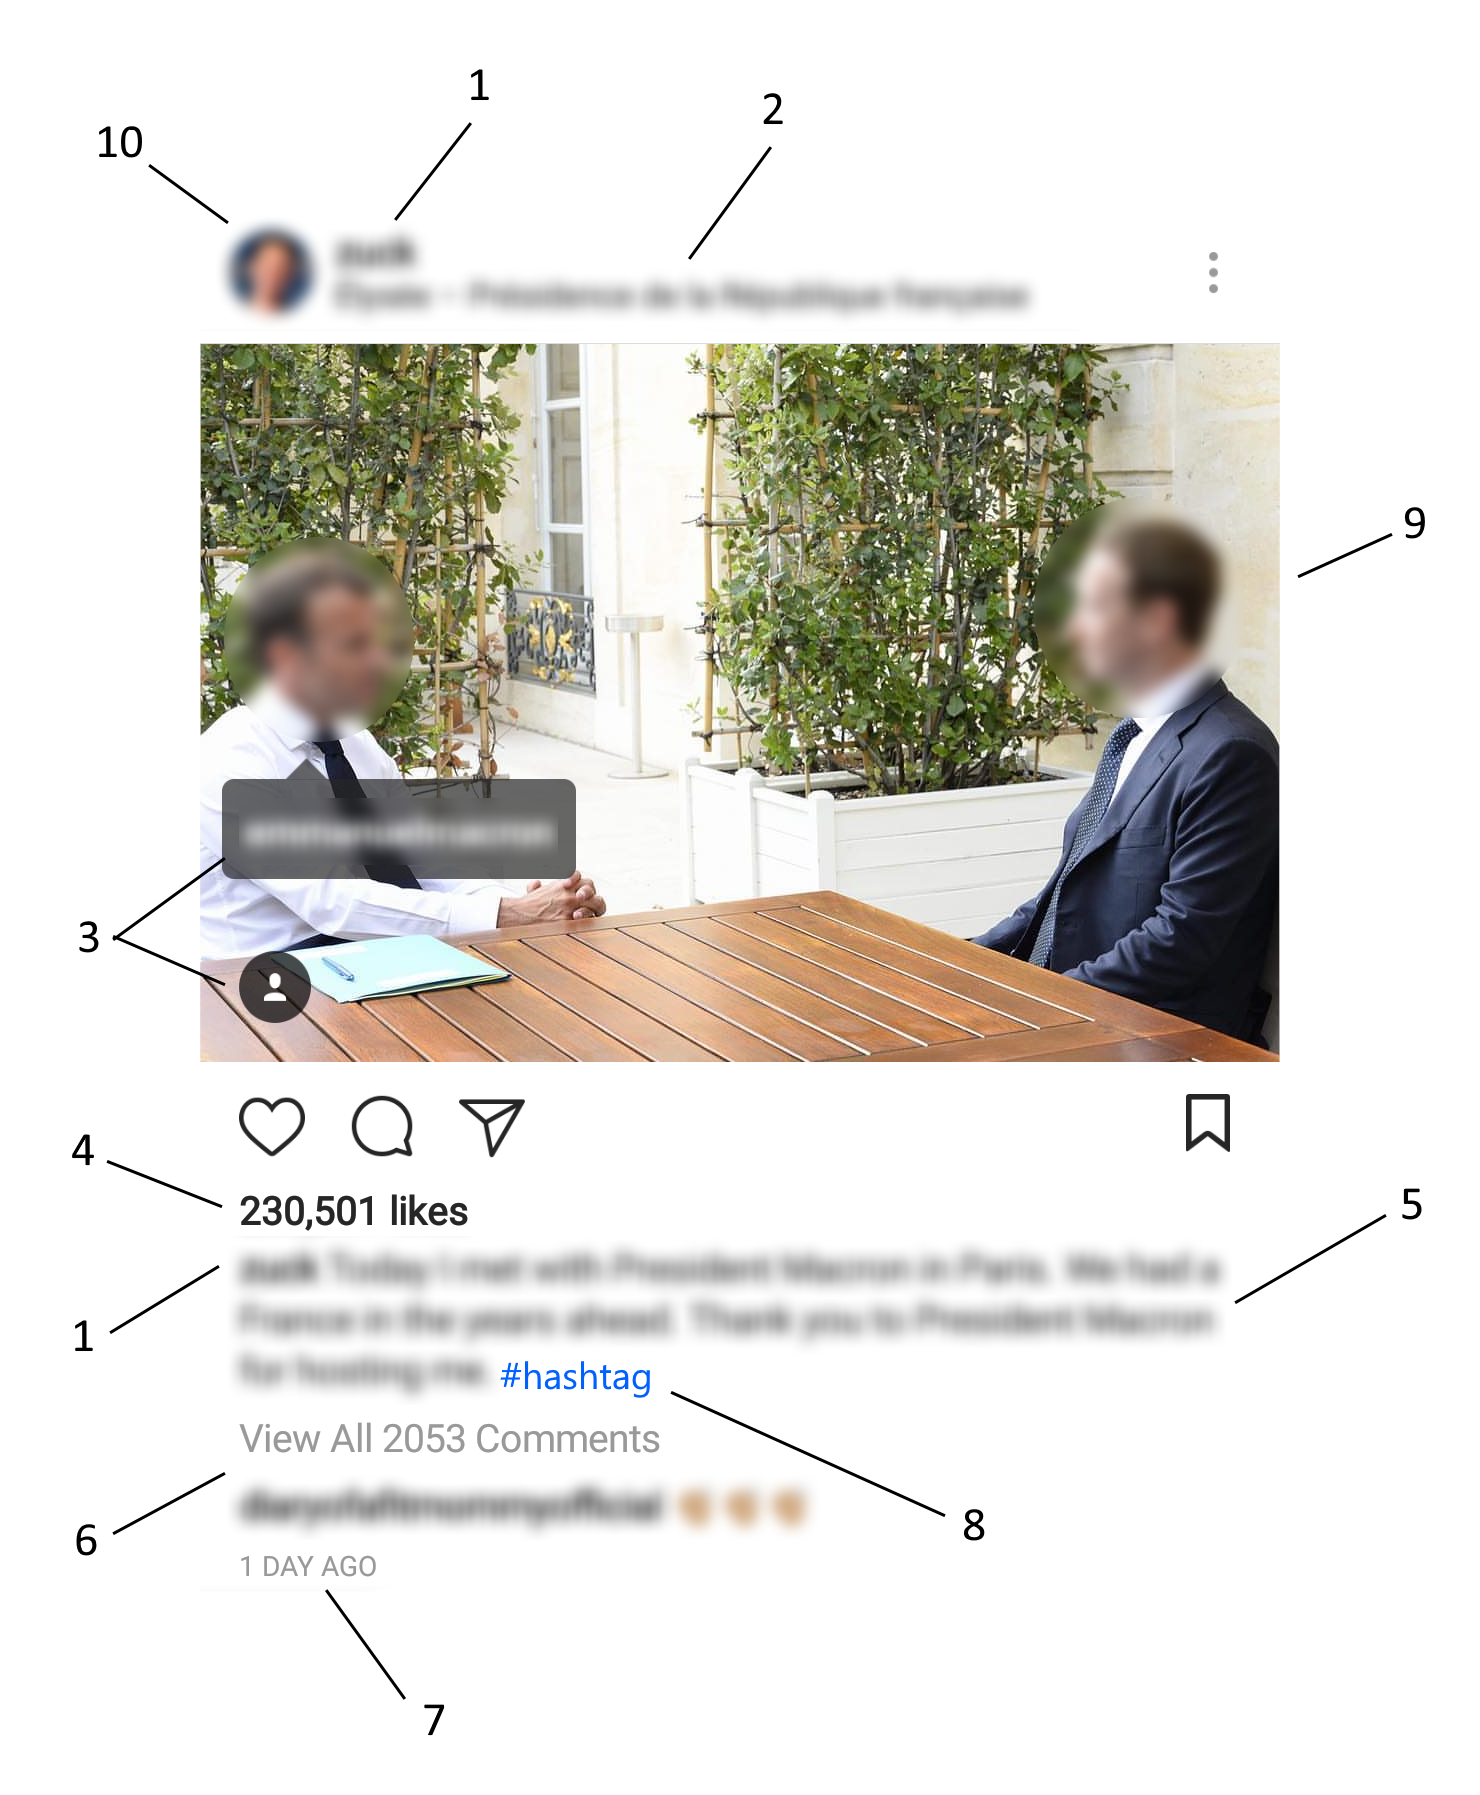
\includegraphics[width=1.0\linewidth ]{Projectdoc/Assets/Illustrationer/IG-meta.png} 
            \caption{Et eksempel på en større mængde metadata på et Instagram opslag}
            \label{fig:ig_metadata}
        \end{figure}
    \end{minipage}
    \begin{minipage}{.35\textwidth}
        \begin{enumerate}
            \item Brugernavn
            \item Lokation
            \item Referering til andre konti
            \item "Syntes godt om" tæller
            \item Beskrivelse
            \item Kommentarer
            \item Klokkeslet
            \item Hashtags (Kategorisering)
            \item Medie (Hoved dataen)
            \item Profil billede
        \end{enumerate}
    \end{minipage}
\end{table}

Dette er især sandt på sociale medier, hvor der kan findes en stor mængde af generelle søgeord. Netop det faktum at sociale medier tillader de enkelte brugere, at skabe en varierende mængde af metadata for et hvert billede, sandsynliggør at systemet vil være i stand til at generere disse søgeord med en prædefineret algoritme for hver tråd på forummet. Dette vil så gøre det muligt at søge efter nye opslag på enhver forumstråd. En række eksempler på metadata kan ses i Figur. \ref{fig:ig_metadata}

\subsubsection{Forum struktur}
\label{forum_struktur}
Da et forum kan designes på flere måder, her vil det blive diskuteret hvilken struktur, som vil passe bedst til produktets tænkte anvendelse. Som det kan ses i [Figur \ref{fig:forskellige_fora}] er både Stackoverflow og Jodel fora, men med vidt forskellige formål. Stackoverflow er generelt set anvendt til at løse specifikke problemer. Disse problemer kan så gives relevante søgeord, og kan på den måde opdages af interesserede personer. Der er også kategorier, som samler de nyeste opslag eller mest sete osv.

\begin{figure}[H]
    \begin{subfigure}{0.5\textwidth}
        \centering
        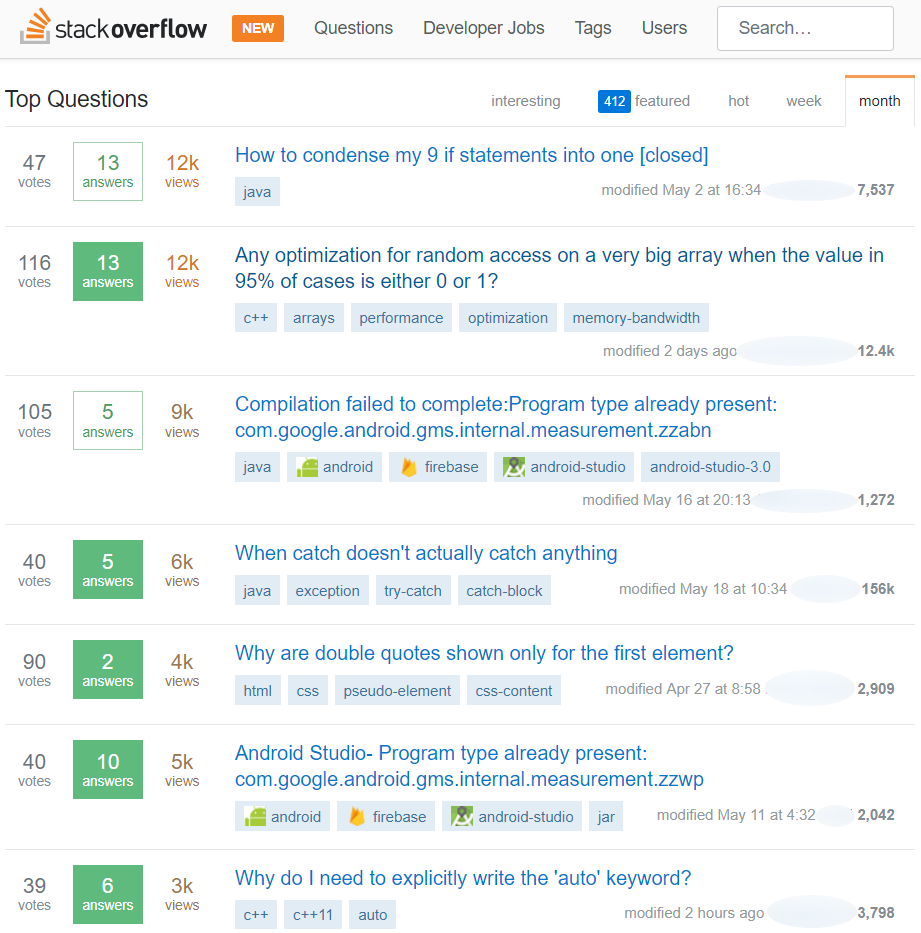
\includegraphics[width=1.0\linewidth ]{Projectdoc/Assets/Illustrationer/stackoverflow_forum_eksempel.png} 
        \caption{Stackoverflows forum struktur}
        \label{fig:stackoverflow_forum}
    \end{subfigure}
    \begin{subfigure}{0.5\textwidth}
        \centering
        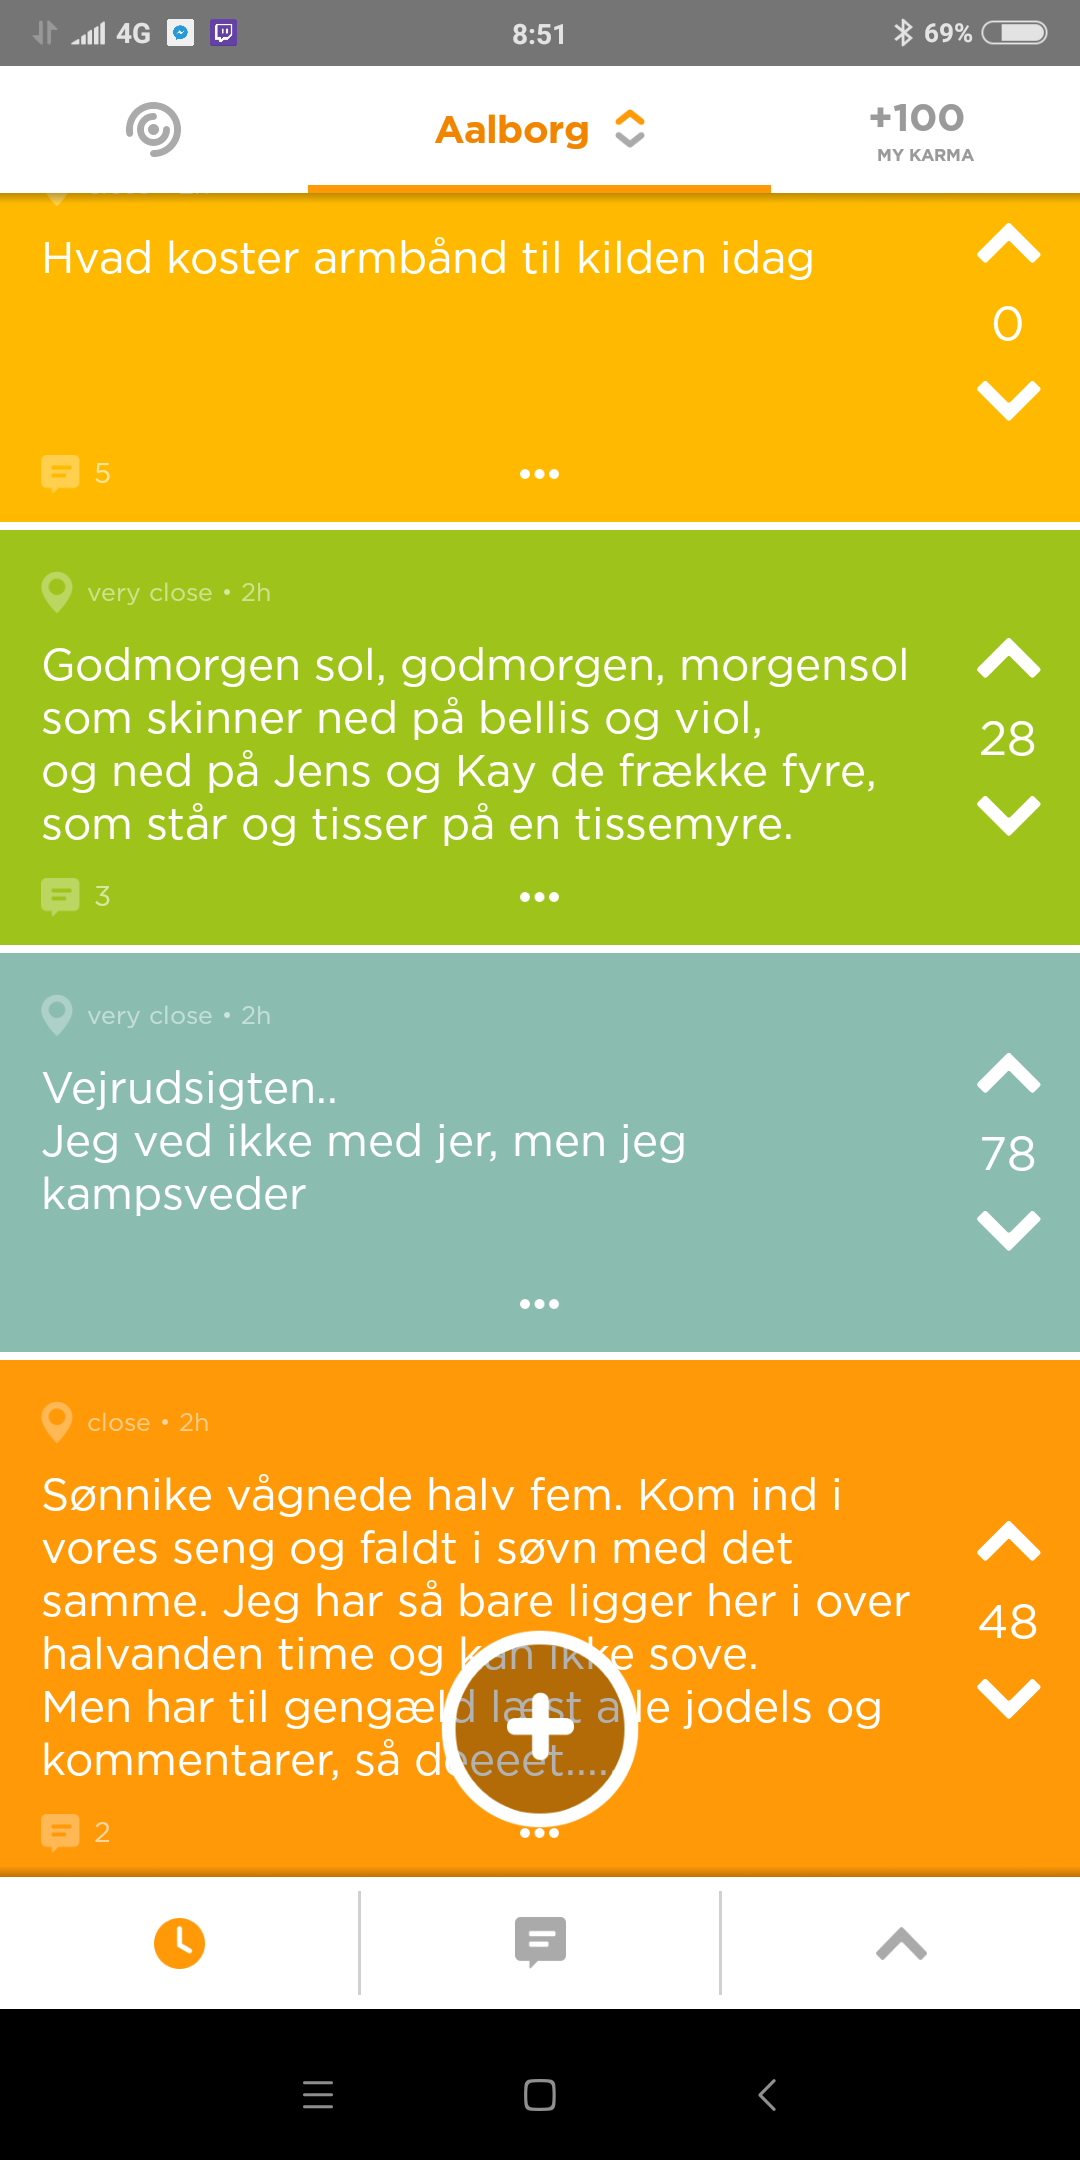
\includegraphics[width=0.7\linewidth]{Projectdoc/Assets/Illustrationer/jodel_forum_eksempel.png}
        \caption{Jodels forum struktur}
        \label{fig:jodel_forum}
    \end{subfigure}
    \caption{Forskellige fora}
    \label{fig:forskellige_fora}
\end{figure}

I kontrast til dette er Jodel en mere ufiltreret, og tilfældig, samling af anonyme opslag. Det eneste der er fælles for opslagene, man ser på Jodel, er at de er inden for en bestemt fysisk radius af hinanden.
Da systemet gerne skulle kunne bruges til seriøse diskussioner om vigtige emner, så virker noget ligende Stackoverflows model værende en bedre idé. Man kunne også forestille sig et "lokalt" nyhedsstørm, som kunne medføre lokations specifikke diskussioner.\\
Hvis disse to funktionaliteter ønskes, vil det kræve to forskellige sammenkædnings algoritmer, da den ene er baseret på lokation, og den anden på tråd. Dette vil give anledning til to potentielt og meget forskellige køretider, der videre vil blive bearbejdet i det næste afsnit.

\subsubsection{Forespørgsler og køretid}
Køretiden på systemets forespørgsler afhænger af flere faktorer, nogle af disse værende:\\ 
Mængden af de forespørgsler systemet laver til det sociale medie, tiden det tager at behandle den modtaget data samt trejdepartens systems køretid. \\
Hvoraf den sidstnævnte er uafhængig af systemet selv, og kan derfor ikke optimeres yderligere i fra internt perspektiv. Det kan forespørgsel algoritmen derimod godt. 

\begin{figure}[H]
    \begin{subfigure}{0.5\textwidth}
        \centering
        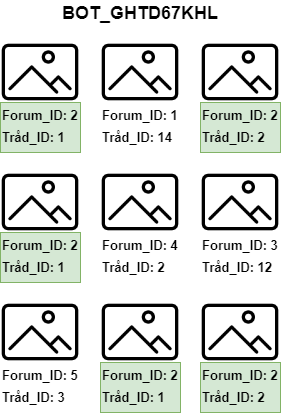
\includegraphics[width=0.70\linewidth]{Projectdoc/Assets/Illustrationer/bot-structure-1.png}
        \caption{Hver bot kan lagre fra alle fora}
        \label{fig:bot_unstructured}
    \end{subfigure}
    \begin{subfigure}{0.5\textwidth}
        \centering
        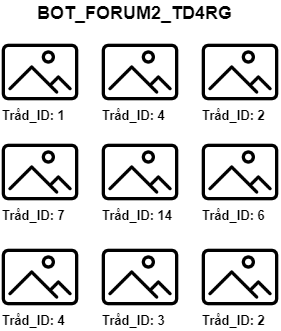
\includegraphics[width=0.70\linewidth]{Projectdoc/Assets/Illustrationer/bot-structure-2.png}
        \caption{Hver bot har eget forum}
        \label{fig:bot_structured}
    \end{subfigure}
    \caption{2 eksempler på bot strukturer, på højre hånd eftersøges der kun opslag fra forumet med ID'et 2 (markeret med grøn).}
    \label{fig:bot_structure}
\end{figure}

\textbf{Optimering af forespørgslerne}\\
Når en bruger af systemet vil navigere til et specifikt forum, vil der blive sendt en forespørgsel til alle de relevante bots, som lagrer opslaget. Systemet søger nu efter et specifikt stykke metadata, som kun systemet vil kunne genkende, og som uvidende personer dermed ikke kan tyde med det blotte øje. Det første stykke information systemet leder efter er et \textit{forum ID}, der henter alle opslag tilknyttet det ønskede forum. Det har potentiale til at være rigtig mange forespørgsler for at genere en forumsoversigt. Systemet kigger derfor også efter et \textit{tråd ID}, som bruges til at holde styr på den individuelle tråds struktur, forstået som rækkefølgen på opslagene i tråden [Visualiseret på Figur \ref{fig:bot_unstructured}].\\
Systemet henter i første gennemsøgning kun det første opslag fra alle \textit{forum ID} med et unikt \textit{tråd ID}. Det vil sige at gennemsøgning kun henter den indledende opslags tråd, og ignorerer andre opslag af samme \textit{tråd ID}. De resterende opslag fra de individuelle tråde bliver først alle hentet når en bruger navigerer sig ind på trådens hovedopslag. Denne metode benyttes for at mindske antallet af forespørgsler til det sociale medie, både for at optimere indlæsnings tiden, men også til at mindske chancen for at blive opdaget pga. denne store mængde mistænkelig data trafik.
\\\\
En måde hvorpå man kunne mindske søgningerne yderligere, er ved at oprette bots, som er kædet sammen med et og kun et forum [Visualiseret på Figur \ref{fig:bot_structured}]. Det vil sige at behovet for et \textit{forum ID} helt forsvinder, da alle opslag er samlet på de relevante bots. Der er dog nogle ulemper ved den løsning, blandt andet så vil dette forværre skalerbarheden, da systemet ikke bare kan blive udvidet med en ny bot, til at klare belastningen fra for eksempel to fora, med denne løsning ville dette kræve to separate bots. Løsningen kan også rydde et helt forum ved nedbrud, men den førnævnte vil kun miste en vis mængde opslags kontekst. Selv med disse ulemper vil den potentielle køretids optimering overgå disse mindre hindringer. Brugen af \textit{tråd ID'et} forbliver det samme.

\subsubsection{Private beskeder (Brug af unikt hash)}
\label{privatbesked}
En feature der vil kunne tilbyde yderligere sikkerhed, for bestemte typer af brugere og brugsmål, er muligheden for at sende private beskeder. For at kunne tillade brugere at kommunikere privat til hinanden, er en unik identifikations bestemmelse, for begge brugere, strengt nødvendigt. Systemet kan derfor ikke tildele en offentlig bot konto for denne aktivitet, da det ikke er realistisk for systemet, at tilegne en unik bot til hver bruger af systemet.\\
For at en feature som denne kan realiseres, vil det kræve at brugeren selv opretter eller tilknytter sin konto fra det pågældende sociale medie. Dette giver systemet adgang til at lagre den hemmelige besked på brugerens konto, hvor kontoens unikke bruger ID fra det sociale medies database nu kan bruges til identifikations bestemmelse. Systemet anvender bruger ID i en hashing algoritme til at genere en, for systemet, læsbar adresse, der også vil kunne deles indbyrdes mellem de der ønsker at sende privat til hinanden. Kun systemet kan oprette og genkende disse hash-koder, til at samle og der ved danne en privat gruppechat. Denne hash genkendelse kunne også udvides til at supportere flere forskellige sociale netværk ad gangen, såfremt systemet har en metode til at kende forskelen på diverse sociale netværk.
\\\\
\textbf{Brug af brugerkonti i hele systemet}\\
Et system baseret på brugernes login i samarbejde med system kontrollerede konti, har også været en overvejelse. Systemet går ud på at brugeren opretter forum opslag fra systemet, der efterfølgende ligger den hemmelige besked i et billede på brugerens egen profil. Problemet ved dette er dog, at sådan system vil kræve et stører dobbelt arbejde fra systemet, da systems bots kun holder styr på beskedens lokation. Det vil sige at systemet først skal sende en forespørgelse til alle de aktive bots, som så her efter forespørger den enkelte brugers profil. Et af fordelene var dog, at systemet kunne kæde brugerne sammen med de opslag de lavede, selvføjelig med et anonymiserende hash. Det kasserede system er beskrevet yderligere i appendix \ref{userbased}.

\subsection{Opsummering af alle overvejelserne}
\label{Opsummering_Overvejelserne}
Ud fra de overstående overvejelser og metoder, kan et endeligt system dannes som følgende struktur:

\begin{figure}[H]
    \centering
    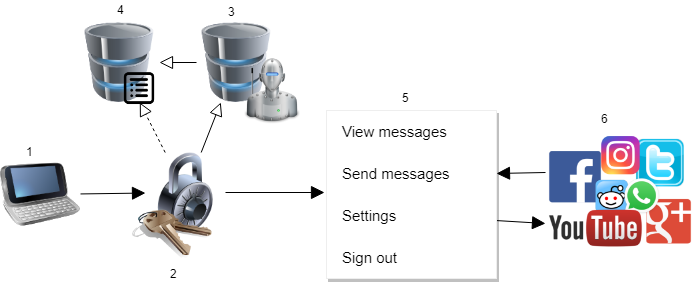
\includegraphics[width=0.70\linewidth]{Projectdoc/Assets/Illustrationer/System_struckure.png}
    \caption{System}
    \label{fig:sysdiagram}
\end{figure}

Systemets struktur beskriver, en central database [Figur \ref{fig:sysdiagram}.4] indeholdende information om alle systemets mindre databaser [Figur \ref{fig:sysdiagram}.3], der kan eksistere i uvist eller dynamisk antal, og videre indeholder informationer til anonyme brugere, om de aktive bots, der er dynamisk genereret til de enkelte sociale medier.\\
Denne centrale database er herved kun tilgået fra slutenhederne, når de ikke længere kan tilgå enkelte mindre databaser, symboliseret i [Figur \ref{fig:sysdiagram}.2, \ref{fig:sysdiagram}.3 og \ref{fig:sysdiagram}.4] med en stiplet linje, og har derfor ingen direkte forbindelse til omverdenen, ud over de enkelte enheder.\\
Den centrale database kræver kun vedligeholdelse af dens indhold, men til gengæld kræver de mindre databaser opsætning for hver gang de opdateres, og efter eventuelle lukninger fra sociale medier. Her vil de falske konti selv også kræve det samme.
Enhederne [Figur \ref{fig:sysdiagram}.1] kan herefter selv hente information, fra disse mindre databaser, nødvendigt for at danne beskederne, og til sidst også selv poste eller hente beskeder, samt besked tråde, til og fra de sociale medier.